\subsubsection{Deep Learning Architectures}

Generative \ac{DL} architectures establish blueprints for developing \ac{DL} networks that synthesize diverse and novel data samples according to a learned distribution. These architectures entail creating latent data constructs and learning to emulate the fundamental statistical patterns found in observed data.

Generative deep neural models have been applied to tasks comprising image synthesis, text generation, and audio synthesis. Their popularity has recently surged owing to their remarkable ability to generate high-quality data and effectively model complex distributions. In the following sections, we outline the most ordinarily used generative \ac{DL} architectures, presented chronologically, as summarized in Table~\ref{tab:archs}.

\begin{table*}[ht]
\centering
\caption{Comparison of Generative Deep Learning Architectures}
\label{tab:archs}
\begin{tabularx}{\textwidth}{|p{20mm}|c|p{25mm}|X|c|}
\hline
\textbf{Model} & \textbf{Year} & \textbf{Type} & \textbf{Key Characteristics} & \textbf{Inference} \\ \hline
DARN & 2013 & Autoregressive & Uses a single model to predict the probability distribution of each output token conditioned on the previous tokens & Sequential \\ \hline
VAE & 2013 & Variational Autoencoder & Learns a latent representation of the input data and generates new samples by sampling from the learned latent space & Parallel \\ \hline
GAN & 2014 & Generative Adversarial Network & Consists of a generator and a discriminator that compete in a two-player minimax game to generate realistic samples & Parallel \\ \hline
Normalizing Flows & 2015 & Flow-based models & Transforms a simple probability distribution into a complex one by applying a sequence of invertible transformations & Parallel \\ \hline
Diffusion & 2015 & Flow-based models & Uses a diffusion process to model the probability distribution of the data & Parallel \\ \hline
Transformers & 2017 & Attention-based models & Uses self-attention to capture global dependencies and generate sequences & Sequential \\ \hline

VQ-VAE &
    2018 &
    Variational Autoencoder &
    Discretizes the continuous latent space by mapping each latent vector to the closest codebook vector &
    Parallel \\ \hline

MS-VQ-VAE &
    2019 &
    Variational Autoencoder &
    Is an extension of the VQ-VAE that incorporates multiple discrete latent spaces of different scales, enabling hierarchical and diverse representations with improved abstraction levels and latent space expressiveness &
    Parallel \\ \hline

\end{tabularx}
\end{table*}

This section will discuss novel architectural designs for \ac{DL}. It is important to note that there is a discrepancy between the date of their conceptualization and their widespread adoption. This trend is common in machine learning because software theories have a faster rate of development compared to hardware theories.

This section does not describe all \ac{DL} architectures that had some relevance. It, however, describes the ones used either by the models developed or by systems studied for the state-of-the-art.

\paragraph{Feedforward Neural Network (1957)} \label{sec:feedforward}

To understand \textit{feedforward neural networks} (or any neural network), it is essential to understand both Hebbian learning and the perceptron.

In 1949, inspired by the observation that neurons that fire together wire together, the psychologist Donald Hebb \cite{hebb_organization_1949} developed a rule for adjusting the strength of connections between neurons in any neural network. The rule goes by the name of Hebbian learning and states that if two neurons are activated simultaneously, their connection should be strengthened. The idea behind Hebbian learning is that learning occurs as a result of changes in the strengths of synaptic connections between neurons in the brain rather than solely due to changes in the activity of individual neurons.

The perceptron is a simple model first published in 1958 by F. Rosenblatt \cite{rosenblatt_perceptron_1958}. It consists of a single neuron with a binary threshold --- also known as bias --- and is used for binary classification tasks. A set of weights transforms the input to the perceptron. The output is determined by checking if the input is enough to trigger the bias and then applying a function to the weighted sum of inputs as shown in Figure \ref{fig:perceptron}. The output of the perceptron can be mathematically expressed as in the equation \ref{eq:perceptron-ouput}.

\begin{equation} \label{eq:perceptron-ouput}
    y = h(\sum_{x=1}^N (I_x \times W_x) - b)
\end{equation}

$y$ is the output, $N$ is the number of inputs, $I_n$ is the input number $n$, $W_n$ is the weight related to $I_n$, $b$ is the bias, and $h$ is an activation function, usually.

The perceptron is trained using an algorithm that adjusts the weights based on the error between the actual and predicted outputs. The exciting part is that Hebbian learning can be applied to perceptrons, which was one of the bases of the future backpropagation. The perceptron can only classify linear separated sets, as shown in \textit{Perceptrons} \cite{marvin_minsky_perceptrons_1969}, hence the need for more complex structures.

\begin{figure}[ht]
    \centering
    \ctikzfig{figures/2-sota/perceptron}
    \caption[Perceptron]{\textbf{Perceptron} --- The perceptron receives multiple inputs associated with a weight. It also holds a given bias. Its output is the application of a given function (\textit{e.g.} step function) to the weighted average of the inputs minus the bias.}
    \label{fig:perceptron}
\end{figure}

A feedforward neural network is no more than a set of layers of perceptron-like neurons. In a feedforward neural network, information moves in only one direction --- forward. Hebbian learning no longer applies to these networks, so more complex algorithms, such as backpropagation, are required. These networks are universal approximators \cite{cybenko_approximation_1989} if they have at least one hidden layer, meaning they can approach any function given the proper configuration. They can also learn different tasks than classification, such as regression. The first functional networks, called multi-layer perceptrons, were invented in the 1980s. An example structure of a feedforward neural network can be seen in Figure \ref{fig:feed_forward_neural_network}.

\begin{figure}[!ht]
    \centering
    \ctikzfig{figures/2-sota/feed-forward-neural-network}
    \caption[Feedforward Neural Network]{\textbf{Feedforward neural network} --- The size of the input is constant. The flow of information goes through nonlinear functions on hidden layers. Both weights between nodes on different layers and the nodes' bias are trained with backpropagation.}
    \label{fig:feed_forward_neural_network}
\end{figure}

To a certain extent, since the perceptron is the most basic feedforward neural network (consisting of only one neuron), these networks do not necessarily equate to deep learning (\ac{DL}). Smaller networks have existed and been utilized for decades. Nevertheless, the foundation for most \ac{DL} architectures comes from this, making it essential to recognize.
\paragraph{Convolutional Neural Network (CNN) (1980)} \label{sec:CNN}

During the 1950s and 1960s, Hubel and Wiesel~\cite{hubel_receptive_1959}, who were distinguished neurophysiologists, conducted pioneering research on the eyes of cats. Their research uncovered the presence of neurons with receptive fields that map various visual regions. Receptive fields refer to specific areas in the visual field that activate particular cells. Their studies revealed two fundamental categories of cells involved in visual processing: simple cells with a strong response to edges and complex cells with larger receptive fields that prioritize the organization of edges over their precise positioning.

In 1980, Kinihiko Fukushima introduced the \textit{neocognitron} which marked a significant milestone in the development of \acp{CNN} \cite{fukushima_neocognitron_1980}. It was one of the first \ac{CNN} architectures designed to mimic specific aspects of human visual perception. This laid the groundwork for future advances in deep learning for computer vision tasks.

\Acp{CNN} are a category of \ac{DL} neural networks widely used in computer vision and other sequential data types. The architecture of \acp{CNN} is specifically designed to handle inputs where data correlate with its vicinity.

The key idea behind \acp{CNN} is to learn and extract features from the input hierarchically. This is achieved through convolutional layers, where a small set of learnable filters are used to scan and transform the input image into a feature map. These networks also use pooling layers that perform down-sampling of the feature map to reduce its size while retaining important information. These operations allow the network to capture patterns and features in the input, which can then be passed to feedforward neural networks and used for classification or regression. This process is represented in Figure \ref{fig:cnn}.

\begin{figure}[ht]
    \centering
    \ctikzfig{figures/2-sota/cnn}
    \caption[Convolutional Neural Network]{\textbf{\Acf{CNN}} --- The network present in the Figure deals with 2D data, such as images. The networks' first step consists of convolutional (and pooling) layers. This first step is responsible for finding features. The deeper the convolutional layer, the bigger the receptive field; consequently, the more abstract the feature. After the features are caught, the flatten operation transforms the data into a 1D vector. And then, the network is no more than a feedforward neural network to, in this case, classify what was fed to the network.}
    \label{fig:cnn}
\end{figure}

A major benefit of \acp{CNN} compared to other kinds of networks is their ability for parallelism, where a long input sequence can be handled fast \cite{huzaifah_deep_2021}. This can greatly accelerate training since the whole output can be processed in one forward pass. The shared weights and local connectivity among neurons in the network enable efficient computation, and using pooling layers lowers the number of parameters to be learned.
\paragraph{Convolutional Operations} \label{sec:conv-layers}

This section will discuss three common layers in \acp{CNN}: convolutional layers, pooling layers, and transposed convolutions. It also introduces the concept of masked convolutions and their applications in specific tasks.

\label{sec:conv-layer}

A \textbf{convolutional layer} is a fundamental building block of \acp{CNN} (see Section \ref{sec:CNN}).

At a high level, a convolutional layer applies a set of learnable filters to the input data, extracting local features and patterns relevant to the task. The filters are typically small and slide over the input data, computing the dot product between the filter weights and the input values at each position. This operation is called convolution and can be seen in Figure \ref{fig:conv-layer}.

\begin{figure}[ht]
    \centering
    \ctikzfig{figures/2-sota/conv}
    \caption[Convolutional layer]{\textbf{Convolutional layer} --- The presented diagram depicts a 1-dimensional convolutional layer designed to process an input signal consisting of a single channel and a length of 7. The layer employs a single filter with a size of 3, resulting in an output signal of length 5 and a single channel. Each element of the output signal is produced by convolving the corresponding filter weights with a subset of the input signal. Specifically, the first output element is generated by convolving the filter with the first three elements of the input signal. The filter is then slid along the input signal with a stride of 1, such that each subsequent output element depends on a different subset of the input signal.}
    \label{fig:conv-layer}
\end{figure}

To be more precise, let us consider a 1D convolutional layer that takes an input tensor $X$ of size $C_{in} \times L_{in}$, where $C_{in}$ is the number of input channels and $L_{in}$ is the length of the input sequence. The layer also has $C_{out}$ filters, each of size $C_{in} \times k$, where $k$ is the size of the filter kernel. The output of the layer is a tensor $Y$ of size $C_{out} \times L_{out}$, where $L_{out}$ is the length of the output sequence.

The convolution operation can be expressed as follows:

\begin{equation}
	Y_{c,i} = \sum_{p=0}^{k-1}\sum_{k=0}^{C_{in}-1} X_{k,i+p} \cdot W_{c,k,p} + b_c
\end{equation}

where $c$ is the index of the output channel, $i$ is the spatial index of the output sequence, $p$ is the spatial index of the filter kernel, $k$ is the index of the input channel, $X_{k,i+p}$ is the input value at position $(k,i+p)$, $W_{c,k,p}$ is the weight of the filter at position $(c,k,p)$, and $b_c$ is the bias term for the $c$-th output channel.

The convolution operation is applied independently to each output channel and each spatial location of the output feature map, resulting in a set of feature maps that capture different aspects of the input data. The weights and biases of the filters are learned during training using backpropagation and gradient descent (see section \ref{sec:backpropagation}), optimizing a suitable loss function for the task at hand.

% alskjdaslkjdasld

\label{sec:pooling}

\textbf{Pooling} is a standard operation in \acp{CNN} that reduces the spatial dimensions of the input feature maps while retaining important information. Pooling is typically applied after convolutional layers to gradually reduce the feature maps' spatial dimensions and increase the network's receptive field. There are several types of pooling, including max pooling, average pooling, L2 pooling, and more. Of these, max pooling is one of the most commonly used.

\textbf{Max pooling} works by partitioning the input feature map into non-overlapping rectangular regions, called pooling kernels. For each pooling kernel, the maximum value is selected and used as the output value for that region. The size of the pooling kernel and the stride determine the amount of reduction in the spatial dimensions of the feature map. The stride is the number of pixels that the pooling kernel is shifted horizontally and vertically between each pooling operation. It can be seen in the Figure \ref{fig:pool}

\begin{figure}[ht]
    \centering
    \ctikzfig{figures/2-sota/pool}
    \caption[Pooling layer]{\textbf{Pooling layer} --- The Figure illustrates a $4 \times 4$ input tensor with a single channel. Each colored square in the tensor denotes a single element. The pooling layer partitions the input tensor into non-overlapping $2 \times 2$ regions and applies a pooling function to each region, resulting in a $2 \times 2$ output tensor with a single channel. The number of channels remains unchanged in this scenario, implying that the pooling function is applied separately to each channel of the input tensor, and the resulting output tensor retains the same number of channels as the input tensor. The primary objective of pooling layers is to decrease the spatial dimensions of the input tensor while maintaining the essential features. In this instance, the pooling layer decreases the spatial dimensions of the input tensor by half, resulting in a smaller output tensor. The output tensor is displayed on the right-hand side of the image, where each colored square represents a single element of the output tensor. The colors of the output tensor correspond to those of the input tensor regions from which they were derived.}
    \label{fig:pool}
\end{figure}

Max pooling has several benefits for \acp{CNN}~\cite{riesenhuber_hierarchical_1999}:
\begin{itemize}
    \item It helps to reduce the model's sensitivity to minor variations in the input. This is because the maximum value within each pooling kernel is selected, which is less sensitive to slight variations than taking the average or other statistics.
    \item It can prevent overfitting by reducing the number of parameters in the model. This is because the pooling operation reduces the spatial dimensions of the feature map, reducing the number of parameters in the subsequent layers of the network.
    \item It can increase the network's receptive field by combining the information from neighboring pixels.
\end{itemize}

There are some potential drawbacks to max pooling as well. One is that it can discard some information that may be important for the task. This is because only the maximum value within each pooling kernel is selected, and other information is discarded.

%laskdjl kajsdlkajs ldkja

\label{sec:transpoed-conv}

A \textbf{transposed convolution}, also known as a deconvolution, is a layer that performs the opposite operation of a convolutional layer. It takes an input tensor of size $C_{in} \times L_{in}$ and produces an output tensor of size $C_{out} \times L_{out}$, where $C_{in}$ and $C_{out}$ are the number of input and output channels, respectively, and $L_{in}$ and $L_{out}$ are the input and output lengths.

The transposed convolution applies a set of learnable filters to the input data. However, instead of sliding the filters over the input, it slides them over the output and computes the dot product between the filter weights and the output values at each position. This operation can be seen as an ``unfolding'' of the convolution operation. Hence the name ``transposed convolution''. An example can be seen in Figure \ref{fig:trans-conv}.

\begin{figure}[ht]
    \centering
    \ctikzfig{figures/2-sota/trans-conv}
    \caption[Transpoed convolution]{\textbf{Transposed convolution} --- This illustration shows how a transposed convolution operation works. The input array has three elements $(3, 4, 3)$ and is shown by the dark blue rectangles at the top. The filter array also has three elements $(5, 5, 2)$ and is shown by the green rectangles in the middle. The output array is obtained by sliding the filter over the input array and computing the element-wise products and sums. The stride parameter controls how much the filter moves, which is 1 in this example. The light blue rectangles at the bottom show the intermediate and final output arrays. The intermediate output arrays are $(15, 15, 6, 0, 0)$, $(0, 20, 20, 8, 0)$, and $(0, 0, 15, 15, 6)$. The final output array is the sum of the intermediate output arrays $(15, 35, 41, 23, 6)$. The gray-shaded regions indicate how the filter broadcasts each element in the input array to produce an intermediate output array.}
    \label{fig:trans-conv}
\end{figure}

The transposed convolution can be expressed as follows:

\begin{equation}
	X_{k,i} = \sum_{p=0}^{k-1}\sum_{c=0}^{C_{out}-1} Y_{c,i+p} \cdot W_{c,k,p} + b_k
\end{equation}

where $k$ is the index of the input channel, $i$ is the spatial index of the input sequence, $p$ is the spatial index of the filter kernel, $c$ is the index of the output channel, $Y_{c,i+p}$ is the output value at position $(c,i+p)$, $W_{c,k,p}$ is the weight of the filter at position $(c,k,p)$, and $b_k$ is the bias term for the $k$-th input channel.

Like convolutional layers, the weights and biases of the filters are learned during training using backpropagation and gradient descent.

\label{sec:masked-conv}

A \textbf{masked convolution} is a convolutional layer that selectively masks out specific input values based on their position in the input sequence. This masking is typically done by setting the weights of the filters to zero for certain positions in the kernel. For example, in an \ac{AR} language modeling task, where the goal is to predict the next word in a sentence given the previous words, a masked convolution can ensure that the model only has access to the previous, not the future words.

Another example where masked convolutions can be helpful is in audio generation tasks. In such tasks, the model takes as input a sequence of audio samples and generates a new sequence of samples that sound similar to the input. In some cases, generating audio that only depends on the previous time steps rather than the entire input sequence may be desirable. This can be achieved using a masked convolution that masks out the future time steps by setting the filter weights to zero for those positions in the kernel. By doing so, the model can only rely on the previous time steps to generate the following sample.

Masked convolutions can be implemented using standard convolutional layers with appropriate masking of the filter weights. Another approach is using a specialized masked convolutional layer that takes an additional mask tensor as input, indicating which input values should be masked.

One advantage of masked convolutions is that they can help prevent the model from overfitting to the training data by forcing it to rely on the input data available at each time step rather than the ground truth values that may not be available at test time. This can be particularly useful in tasks where the input data has a sequential or temporal structure, and the model needs to make predictions based on partial information.

\paragraph{Recurrent Neural Network (RNN) (1986)} \label{sec:rnn}

In 1986, Rumelhart and McClelland, psychologists, in the aftermath of the discovery of the backpropagation algorithm, wrote a book \cite{rumelhart_parallel_1986} where, between others, they took the declarations made in Perceptrons \cite{marvin_minsky_perceptrons_1969}, presented in Section \ref{sec:context}, and showed that, although the perceptron alone might not be enough, networks of perceptrons, with the suitable algorithms, might suffice.

One example they gave was a theoretical network that would be recursive \cite{rumelhart_learning_1987}. This would be the first time the ``recurrent'' term would appear in the literature. They explained that a recursive network is a feedforward network where some weights are kept the same between layers. They showed that it is easy to backpropagate the error and train such a network with this simplification. At the time, ``the major problem with this procedure is the memory required''. This new network was able to solve problems related to sequences. In this chapter, they showed the development of a system that would learn to complete straightforward sentences using \aclp{RNN}.

Furthermore, a \ac{RNN} used nowadays is not very different from the one theorized in 1986. A \ac{RNN} is a neural network derived from a feedforward neural network (see Section~\ref{sec:feedforward}), where some connections between nodes can create cycles. This is because some nodes' output is the same nodes' input. This operation makes the network have memory. These networks can exhibit temporal behavior and process variable-length sequence of inputs. In 1996 it was shown that \acp{RNN} could perform any operation that a regular computer can, meaning that they are Turing complete \cite{hyotyniemi_turing_1996}.

\Ac{RNN} have the problem of forgetting terms seen long ago as new terms come along~\cite{hochreiter_long_1997}. This may be a problem in, for instance, long texts where the model has to remember the name of a given entity that was given at the beginning of the text.

Learning happens as in feedforward neural networks with one additional step: the recurrent nodes are unrolled, as seen in Figure \ref{fig:rnn}.

\begin{figure}[!ht]
    \centering
    \ctikzfig{figures/2-sota/rnn}
    \caption[Simple recurrent neural network]{\textbf{Simple \acl{RNN}} --- The left side of the image displays the most straightforward representation of a \ac{RNN} because it only has one recurrent neuron. Apart from the bias, the neuron has an input weight, a weight for the recursive connection, and a weight for the output. The images on the left and the right are equivalent. The image on the right represents the same simple network. However, it shows what exactly happens when it receives multiple inputs: an output is generated for each one, and a value is passed to the next iteration. One may notice that even though the inputs and outputs change, the weights on the edges do not.}
    \label{fig:rnn}
\end{figure}

New takes that solve the problems with \acp{RNN} have been developed over the years. The basis of these models is to include learnable gates that choose what and when to remember and to forget. The most prominent examples are the \Acfp{GRU} \cite{cho_properties_2014}, and the \Acfp{LSTM} \cite{hochreiter_long_1997}.
\paragraph{RNN Variants} \label{sec:rnn-variants}

\Acp{RNN} are a class of neural networks designed to handle sequential data. They work by maintaining an internal state or memory, which allows them to process sequences of inputs and produce outputs that depend on previous inputs. This definition allows for other types of networks, different from the one shown in the previous section.

However, there are convincing reasons to investigate architectures beyond the basic approach. The typical \ac{RNN} is not without its difficulties, particularly the development of the \textit{vanishing gradient problem} as a major concern.

\Acp{RNN} may be prone to the vanishing gradient problem due to their method of updating internal states. \Acp{RNN} compute the internal state at time step $t$ by incorporating the input of time step $t$ and the previous state of time step $t-1$. This process generates a sequence of dependencies between the present and past states, which leads to multiple matrix multiplications during the backpropagation.

As the gradient keeps decreasing after each multiplication, it may ultimately shrink to such an extent that the neural network fails to learn long-term patterns present in the input sequence.

The prime example of an architecture that fights the vanishing gradient problem is the \textbf{\acf{LSTM}} \cite{hochreiter_long_1997}. \Acp{LSTM} were introduced in 1997 and have since become a popular choice for processing sequential data, especially in \ac{NLP}.

The main idea behind \ac{LSTM} is to introduce memory cells that can selectively forget or remember information from previous time steps. Each memory cell has three gates: the input gate, the forget gate, and the output gate, which control the flow of information into and out of the cell. One can see how these work in Figure \ref{fig:lstm}.

\begin{figure}[ht]
    \centering
    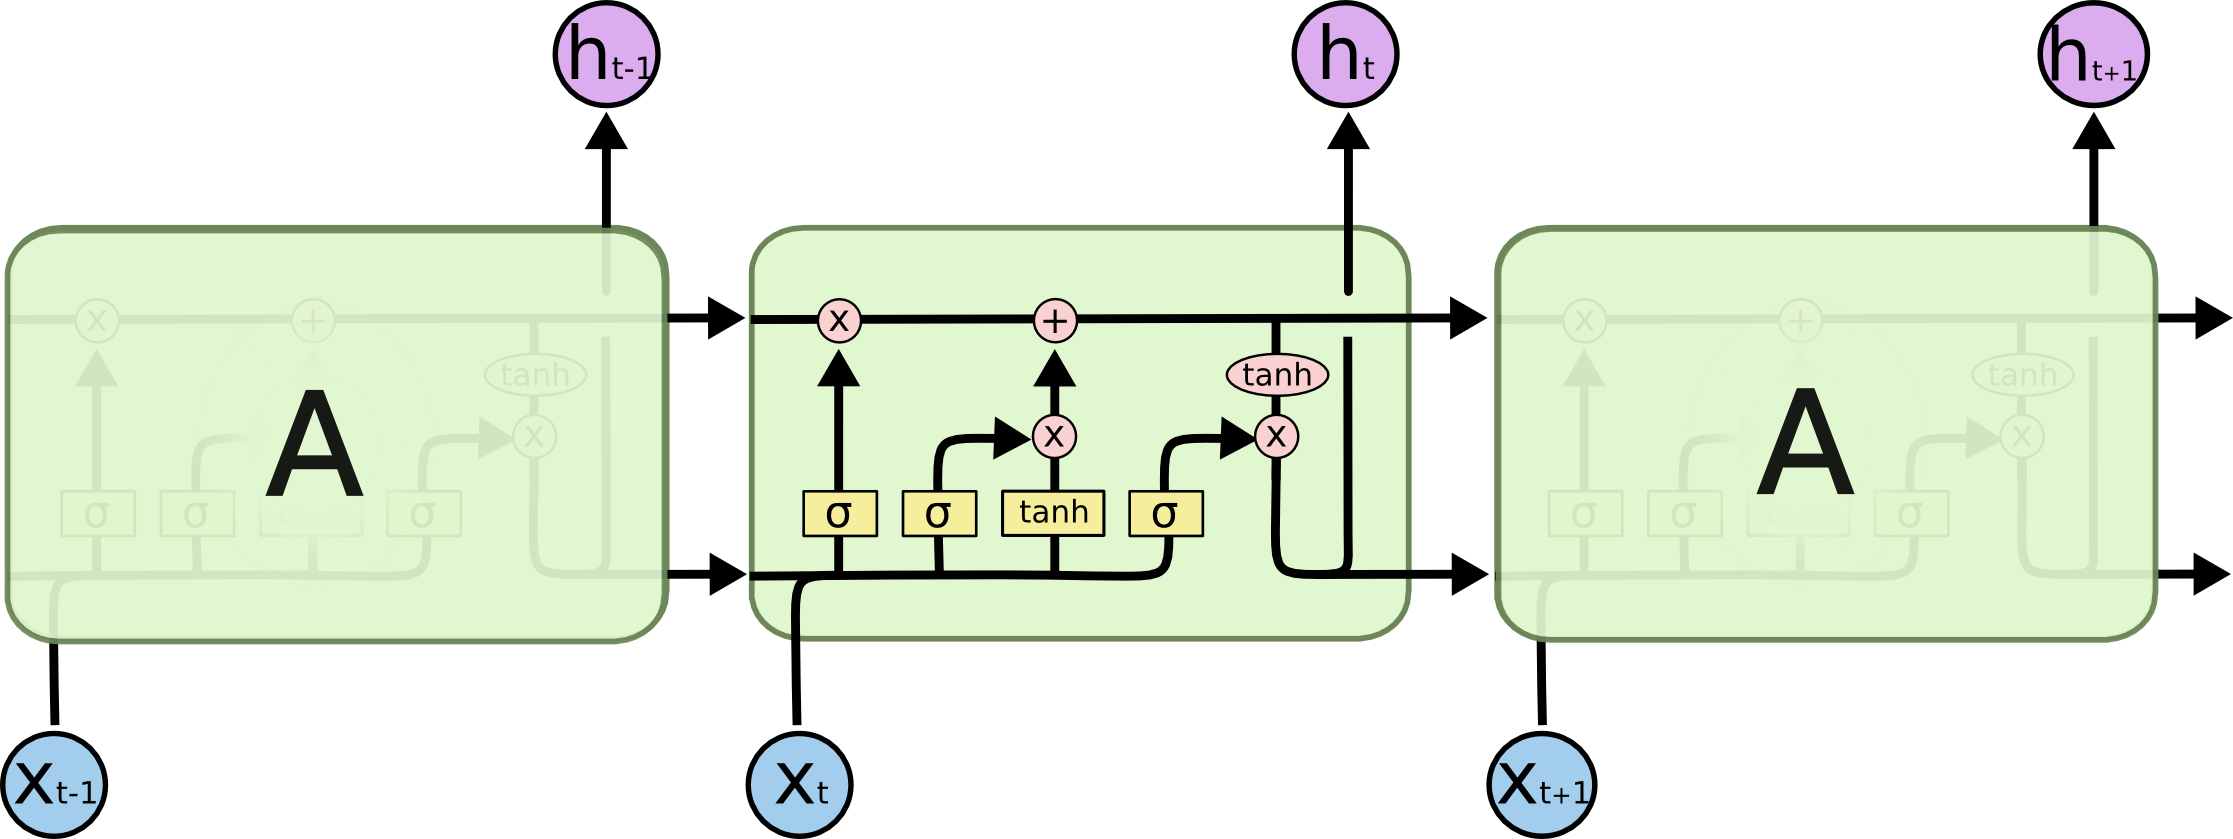
\includegraphics[width=\textwidth]{figures/2-sota/LSTM3-chain.png}
    \caption[Long Short-Term Memory]{\textbf{\Acf{LSTM}} --- 
    The network was taken from \cite{christopher_olah_understanding_2015}. Each green rectangle is an \ac{LSTM} cell. The blue circles represent an input at a given time, such that $X_t$ is the input at time $t$. The pink circles represent the output at a given time $h_t$. Each \ac{LSTM} cell takes three inputs: the previous cell`s memory and output, and the current input, and outputs both the real output and the current memory. In the Figure, the top exiting arrow corresponds to the memory, while the bottom corresponds to the output. The yellow rectangles have learnable parameters, weights, and biases.}
    \label{fig:lstm}
\end{figure}

The forget gate determines which information from the previous state should be forgotten or retained. It takes the current input, $X_t$, and the previous state, $H_{t-1}$, and computes the gate activation, $f_t$, a number between 0 and 1 that determines how much of the previous state should be retained or forgotten. It is calculated as

\begin{equation}
    f_t = \sigma (W_f * [H_{t-1}, X_t] + b_f)    
\end{equation}

$W_f$ is the weight matrix for the forget gate, and $b_f$ is the bias vector.

The input gate determines which information from the current input and the previous state should be allowed into the cell. It takes the current input, $X_t$, and the previous state, $H_{t-1}$, as inputs and computes the gate activation, $i_t$, which is a number between 0 and 1 that determines how much of the input and previous state should be allowed into the cell. It is calculated as

\begin{equation}
    i_t = \sigma (W_i * [H_{t-1}, X_t] + b_i)
\end{equation}

where $\sigma$ is the sigmoid activation function, $W_i$ is the weight matrix for the input gate, and $b_i$ is the bias vector.

The memory update computes the new information stored in the memory cell. It takes the current input, $X_t$, and the previous state, $H_{t-1}$, as inputs and computes the new candidate memory content, $\tilde{C_t}$. It is calculated as

\begin{equation}
    \tilde{C_t} = \tanh (W_C \times [H_{t-1}, X_t] + b_C)
\end{equation}

$W_C$ is the weight matrix for the candidate memory update, and $b_C$ is the bias vector.

The memory cell stores the current memory content, $C_t$, a combination of the previous and new candidate memory content, as determined by the input and forget gates. It is calculated as

\begin{equation}
    C_t = f_t \times C_{t-1} + i_t * \tilde{C_t}
\end{equation}

The output gate determines which information from the current memory cell should be used as output. It takes the current input, $X_t$, and the previous state, $H_{t-1}$, as inputs and computes the gate activation, $o_t$, a number between 0 and 1 that determines how much of the memory cell content should be outputted. It is calculated

\begin{equation}
    o_t = \sigma (W_o \times [H_{t-1}, X_t] + b_o)
\end{equation}

The hidden state, $H_t$, is computed by applying the output gate to the memory cell. It is calculated as

\begin{equation}
    H_t = o_t \times \tanh (C_t)
\end{equation}

By selectively forgetting or remembering information from previous time steps, \acp{LSTM} can maintain long-term dependencies in the input sequence and avoid the vanishing gradient problem that occurs in vanilla \acp{RNN}.

Other kinds of networks that handle the vanishing gradient problem have been proposed. One example is the \textbf{\acf{GRU}}~\cite{cho_learning_2014}. \Ac{GRU} is very similar to \ac{LSTM}. The main difference between \ac{GRU} and \ac{LSTM} is in their architecture and the number of gates they use to control the flow of information. While the \ac{LSTM} has the three gates mentioned above, \ac{GRU} has two gates: the reset gate and the update gate. The update gate controls how much of the previous hidden state to keep, and the reset gate determines how much of the previous hidden state to forget.

Overall, \ac{GRU} has a simpler architecture compared to \ac{LSTM}, which makes it faster to train and requires fewer parameters. However, \ac{LSTM} is generally considered more powerful and better suited for tasks that require longer-term memory, such as machine translation or speech recognition.

Another widespread helpful \ac{RNN} implementation is the \textbf{bidirectional \ac{RNN}}~\cite{schuster_bidirectional_1997}. Unlike traditional \acp{RNN}, which process input sequences in only one direction, from beginning to end, bidirectional \acp{RNN} process input sequences in both directions, from beginning to end and from end to beginning, simultaneously.

The main idea behind bidirectional \acp{RNN} is to use two separate \acp{RNN}, one that reads the input sequence in the forward direction and another that reads the sequence in the backward direction. The output of the two \acp{RNN} are then combined to produce the final output.

The benefit of using a bidirectional \ac{RNN} is that it allows the network to access both past and future context when making predictions about the current time step.
\paragraph{Autoencoder (AE)} \label{sec:autoencoders}

\Acp{AE} are a type of neural network architecture used for unsupervised learning. Their origin is difficult to precise as the literature is vast and multiple representations of this kind of network started popping up at the end of the 1980s with different names.

The primary goal of \acp{AE} is to learn an efficient representation of the input data by encoding it into a lower dimensional space, known as the bottleneck layer, and then decoding it back to the original dimensions. \Acp{AE} try to learn the identity function. The network learns to minimize the reconstruction error between the input and the reconstructed output.

The architecture of an \ac{AE} typically consists of the encoder and the decoder. The encoder maps the input to the bottleneck layer, while the decoder maps the bottleneck layer back to the original dimensions. These layers can be seen in figure \ref{fig:autoencoder}. The bottleneck layer acts as a bottleneck that restricts the amount of information that can be passed through, forcing the network to learn the most important features of the input data. For instance, if the size of the bottleneck layer were the same as the input and the output, the network would not learn the essential features, as a simple pass-through would suffice.

A simple use case for \acp{AE} is embeddings, for instance, word embeddings. If given multiple sentences, a model learns to transform a word in itself, passing it through a bottleneck layer; in the future, only the values in the bottleneck (the embedding) and the decoder are required to get the original word. Since, ideally, these embeddings are more feature rich than the word itself, these representations are beneficial for \ac{NLP} tasks.

\begin{figure}[ht]
    \centering
    \ctikzfig{figures/2-sota/autoencoder}
    \caption[Autoencoder]{\textbf{\Acf{AE}} --- This \ac{AE} receives an input of size five and tries to learn a way to transform it into itself by passing through a bottleneck of size three. In the initial part, from the input to the bottleneck, an encoder is present, while the second part displays a decoder.}
    \label{fig:autoencoder}
\end{figure}
\paragraph{U-Net (2015)}\label{sec:u-net}

U-Net is a deep learning architecture introduced by Olaf Ronneberger et al. in 2015 for biomedical image segmentation tasks \cite{ronneberger_u-net_2015}. The name \textit{U-Net} comes from the shape of the network, which resembles the letter \textit{U}.

The U-Net architecture consists of two main parts: an encoder path and a decoder path. The encoder path is a typical \ac{CNN} (Section \ref{sec:CNN}) that extracts features from the input image. On the other hand, the decoder path uses upsampling operations to recover the spatial resolution of the feature maps and generate a segmentation mask. Upsampling is the process of increasing the resolution of an image or signal by using, for instance, nearest neighbor interpolation, bilinear interpolation, or transposed convolution (see Section \ref{sec:transpoed-conv}). The U-Net architecture can be seen in Figure \ref{fig:u-net}.

\begin{figure}[ht]
    \centering
    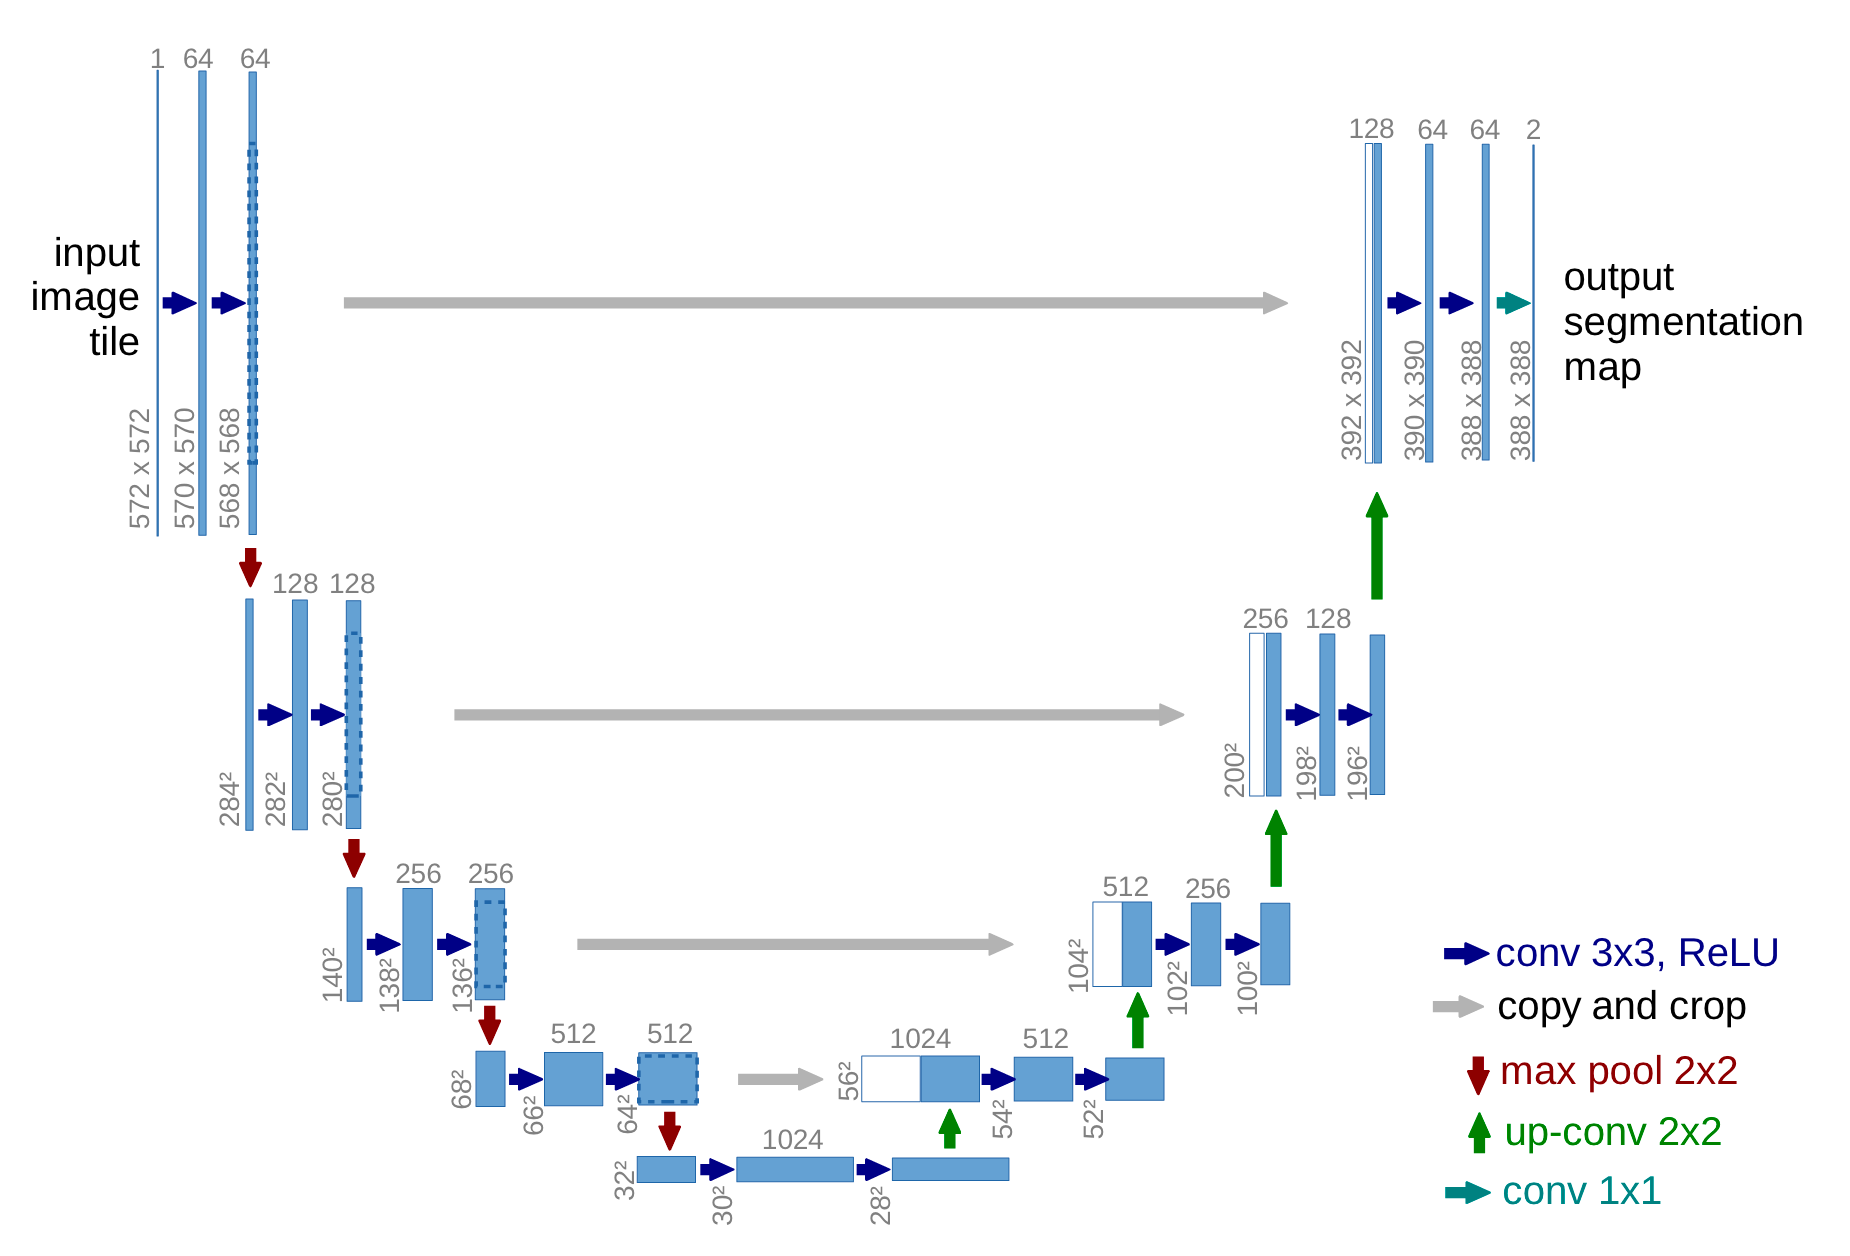
\includegraphics[width=\textwidth]{figures/2-sota/u-net/u-net.png}
    \caption[U-Net]{\textbf{U-Net} --- This figure was taken from the original paper and follows an example for images with $572 \times 572$ pixels. Each blue box corresponds to a multi-channel feature map. The number of channels is denoted on top of the box. The x-y-size is provided at the lower left edge of the box. White boxes represent copied feature maps. The arrows denote the different operations. One can see that at its smallest size, the feature maps were $28 \times 28 \times 1024$, and the end result provides two features maps of $388 \times 388$ pixels, meaning that this specific network could be used, for instance, for segmentation of foreground vs. background. It is also essential to notice that, to keep the original image's fidelity, there is a deconvolutional step for each convolutional one. These are concatenated (represented by the white boxes).}
    \label{fig:u-net}
\end{figure}

The encoder path extracts features from the input image. These features are then compressed into a lower-dimensional representation, which the decoder path uses to generate a segmentation mask for the input image. In this sense, the U-Net architecture can be viewed as a specialized type of \ac{AE} not designed to reconstruct the input image itself.

The U-Net architecture was initially designed to classify each pixel in an image as belonging to a specific object or background: image segmentation. It combines high-level and low-level features from the input image to generate the final segmentation.